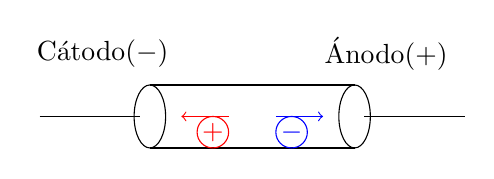
\begin{tikzpicture}
\draw  (-3,0.4) node (v1) {} ellipse (0.2 and 0.4);
\draw  (-0.4,0.4) node (v2) {} ellipse (0.2 and 0.4);
\draw  plot[smooth, tension=.7] coordinates {(-3,0.8) (-0.4,0.8)};
\draw  plot[smooth, tension=.7] coordinates {(-3,0) (-0.4,0)};
\draw [->, blue] plot[smooth, tension=.7] coordinates {(-1.4,0.4) (-0.8,0.4)};
\node at (-3.6,1.2) {C\'atodo($-$)};
\node at (0,1.2) {\'Anodo(+)};

\draw (-4.4,0.4) -- (v1);
\draw (v2) -- (1,0.4);

\draw [blue]  (-1.2,0.2) circle (0.2) node {$-$};
\draw [red]  (-2.2,0.2) circle (0.2) node {$+$};
\draw [->, red](-2,0.4) -- (-2.6,0.4);
\end{tikzpicture}